\documentclass[border=4pt]{standalone}
\usepackage{tikz}
\usetikzlibrary{arrows.meta,positioning,shapes.geometric}

\begin{document}
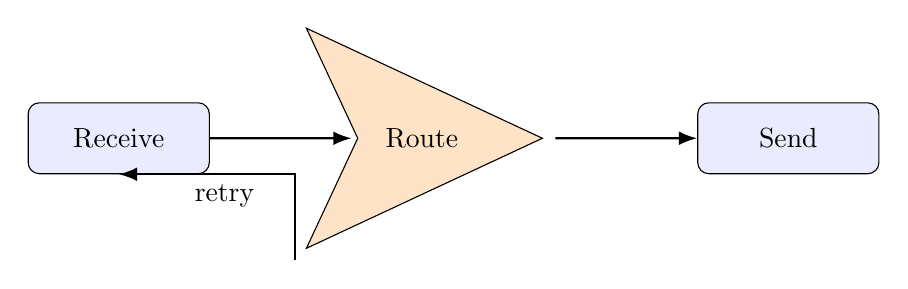
\begin{tikzpicture}[
  >=Latex,
  node distance=18mm,
  process/.style={draw,rounded corners,minimum width=23mm,minimum height=9mm,fill=blue!8},
  dispatch/.style={dart,dart tip angle=50,dart tail angle=130,
    draw,fill=orange!22,minimum width=20mm,minimum height=30mm,outer sep=2pt},
  flow/.style={->,thick}
]
  \node[process] (receive) {Receive};
  \node[dispatch,right=of receive] (route) {Route};
  \node[process,right=of route] (send) {Send};

  \draw[flow] (receive) -- (route);
  \draw[flow] (route.tip) -- (send);
  \draw[flow] (route.right tail) |- node[below,pos=.7]{retry} (receive.south);
\end{tikzpicture}
\end{document}
